\documentclass{article}
\usepackage[utf8]{inputenc}
\usepackage{polski}
\usepackage{graphicx}
\usepackage{hyperref}
\graphicspath{{images/}}

\usepackage{geometry}
\newgeometry{tmargin=4cm, bmargin=4cm, lmargin=3.2cm, rmargin=3.2cm} 

\usepackage{fancyhdr}
\pagestyle{fancy}

 

\begin{document}

\begin{titlepage}
\begin{center}
  
  \LARGE \textsc{Politechnika Wrocławska}\\
  \vspace*{0.2cm}
  \Large \textsc{Wydział Informatyki i Telekomunikacji}\\  
  \vspace*{0.4cm}
  \centering\includegraphics[width=0.2\textwidth]{WITlogo.png}\\
  \vspace*{0.2cm}
  \vspace*{2cm}
        
  \centerline{\rule{\textwidth}{1.2pt}}
  \vspace{0.4cm}
  \Huge\textbf{Klasyfikacja oparta na danych dotyczących ocen gier}
  \centerline{\rule{\textwidth}{1.2pt}}
  \vspace{1cm}
  \LARGE Sprawozdanie z laboratorium\\
  \vspace{3.5cm}
  \textsc{Autor}\\
  \vspace{0.2cm}
  \textbf{Stsiapan Shkliar}\\
  \vspace{0.1cm}
  \Large nr albumu: \textbf{260467}\\
  \vspace{0.1cm}
  kierunek: \textbf{Informatyka Stosowana}
            
            
        
        
  \vspace*{\fill}
  \Large \textit{13 czerwca 2022}
            
 \end{center}


\end{titlepage}

\begin{abstract}
Celem projektu jest predykacja na podstawie danych wcześniejszych ocen czy danemu użytnikowi spodoba się dana gra czy nie. Dane byli pobrane \url{https://howlongtobeat.com} oraz \url{https://www.metacritic.com}. Pobrane dane zostały następnie oczyszczone  do predykcji oceny gry na podstawie jej cech.

\end{abstract}

\section{Wstęp -- sformułowanie problemu}
\label{sec:wstep}

Jaki jest problem?
Autor potrzebuje przewidzieć, czy spodoba się mu ta gra, czy nie. Pozwoli mu to na predykowanie oceny gry oraz czy warto taką grę kupować czy nie...

\section{Opis danych}
Wielkość datasetu 300 wierszy.
Kolumna "Title" - zmienna typu string, okreśła ona nazwę gry. Zbiór wartości: Lumines: Puzzle Fusion, Mr. DRILLER: Drill Spirits, Call of Duty 2, Need for Speed: Most Wanted 5-1-0.

Kolumna "Max Players" - zmienna typu 'int', określa ona maksymalną liczbę graczy.Zbiór wartości:1,2,4.

Kolumna "Multiplatform" - zmienna typu 'boolean', określa ona czy dana gra potrzymuje multiplatform.Zbiór wartości:true,false.

Kolumna "Online" - zmienna typu 'boolean', określa ona czy można grać online w danej grze.Zbiór wartości:true,false.

Kolumna "Genres" - zmienna kategoryczna , okreśła ona gatunek gry. Zbiór wartości: Action,Strategy,Sports,Adventure,RPG.

Kolumna "Publishers" - zmienna kategoryczna, okreśła ona wydawców gry. Zbiór wartości: Nintendo,Ubisoft,EA,Adventure,Konami.

Kolumna "Review Score" - zmienna typu 'int', określa ona ocenę gry.Zbiór wartości:85,89,35,68.

Kolumna "Total Sales" - zmienna typu 'float', określa ona sumę z sprzedaży gry graczy.Zbiór wartości:4.69,0.56,0.41,0.06.

Kolumna "Price" - zmienna typu 'int', określa ona maksymalną liczbę graczy.Zbiór wartości:24.95,29.99,41.99.

Kolumna "ESRB Rating" - zmienna kategoryczna, określa ona ocenę ESRB.Zbiór wartości:E,M,A,RP.

Kolumna "Year of Release" - zmienna typu 'int', określa ona rok wydania gry.Zbiór wartości:2001,2015,2008.

Kolumna "Number Of Players Completed The Game" - zmienna typu 'int', określa ona  liczbę graczy,którzy skończyli grę.Zbiór wartości:57,888,1020.

Kolumna "Completionists Average Time" - zmienna typu 'float', określa ona średnią liczbę godzin zużytych przez gracza dla skończenia gryw calósci.Zbiór wartości:29.766666666666666,1.25,16.383333333333333.

Kolumna "Main Story Average Time" - zmienna typu 'int', określa ona średnią liczbę godzin zyżytych przez gracza dla skończenia głownie częsci gry.Zbiór wartości:14.333333333333334,10.333333333333334,15.5.

Kolumna "Like" - zmienna typu 'int', określa ona czy podoba się dana gra.Zbiór wartości:0,1.

\section{Opis rozwiązania}
Dane zostały stworzone na podstawie znalezionej informacji ze stron \url{https://howlongtobeat.com} , \url{https://www.metacritic.com} oraz opinii użytkownika.
 Baza została zapisana w postaci ramki danych biblioteki \texttt{Pandas}. Zawiera ona informacje o 300 gier wraz z 14 cechami je określającymi.

Używając metody klasyfikacji za pomocą \textit{Neural Neu} na danych uzyskano model pozwajacy na określenie oceny gry na podstawie jego cech.

\section{Rezultaty obliczeń}

\subsection{Plan badań}
Zbiór danych zostanie podzielony na dwie części: treningową i testową w stosunku 80:20. 
\subsection{Metryki używane przy klasyfikacji}
Dokładność (Accuracy)

Metryka poprawności zaklasyfikowanych elementów we wszystkich klasach.

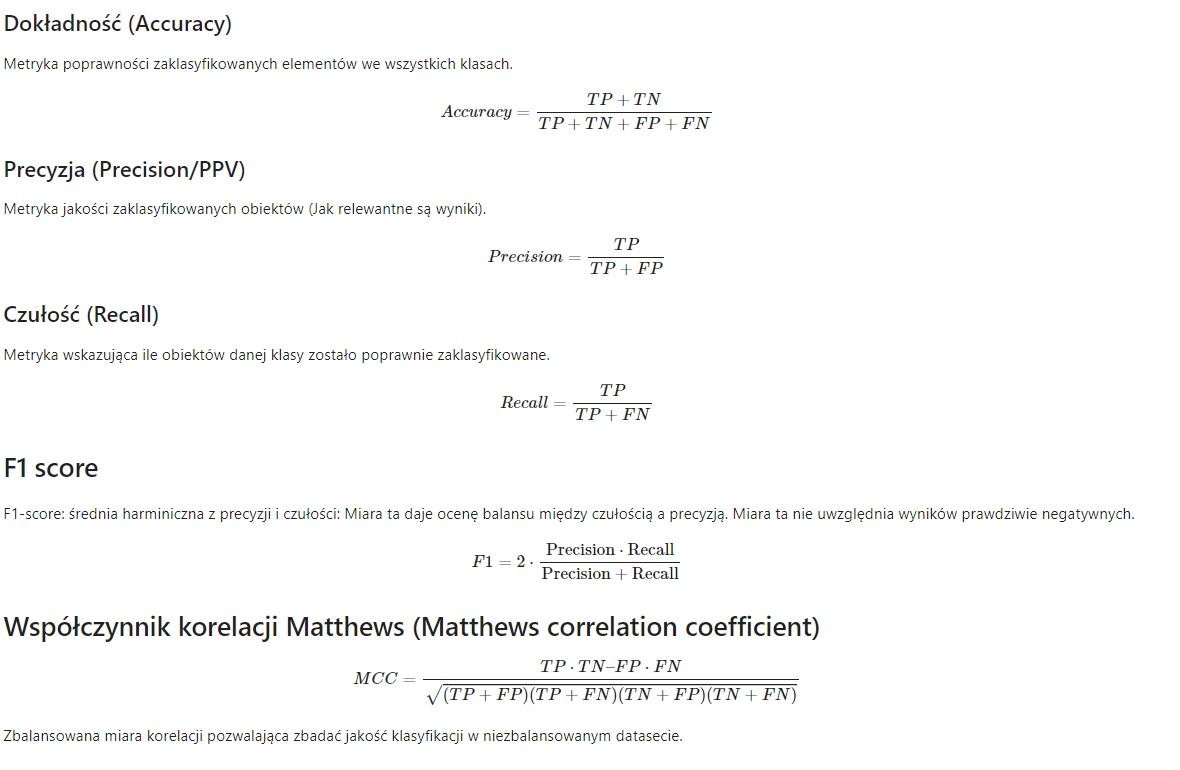
\includegraphics[width=1.2\linewidth]{metryki.png}
\end{center}

\subsection{Wykresy obliczeń} 
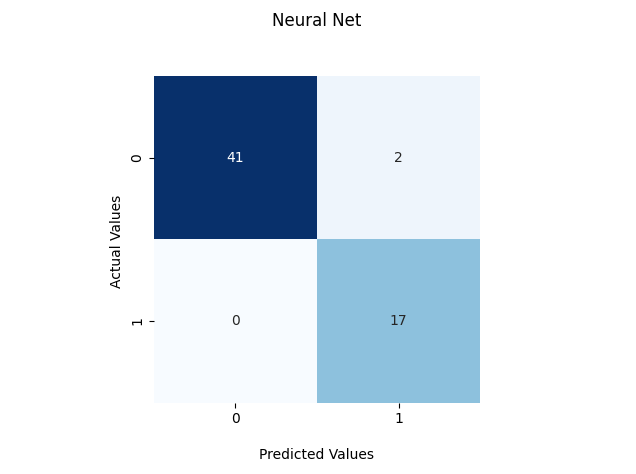
\includegraphics[width=0.8\linewidth]{wykres_1.png}

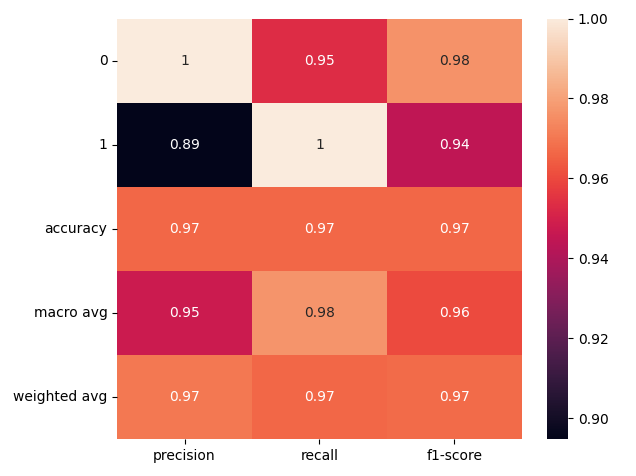
\includegraphics[width=0.8\linewidth]{wykres_2.png}
\end{center}
\end{figure}


\section{Wnioski}
Przedstawiona klasyfikacja działa poprawnie z dobrym procentem dokładności na podstawie danych wcześniejszych ocen,czyli może znaleźć grę,która spodoba się użytnikowi. W przyszłości klasyfikacja ta może zostać rozszerzona na dobry system rekomendacji.


\appendix
\section{Dodatek}
Kody źródłowe(utrzymane w konwencji języka Python wraz z instrukcjmi uruchomienia) umieszczone zostały w repozytorium github:

\noindent \url{https://github.com/nonamestephan/MSID_project}.


\end{document}